%%%%%%%%%%%%%%%%%%%%%%%%%%%%%%%%%%%%%%%%%
% Programming/Coding Assignment
% LaTeX Template
%
% This template has been downloaded from:
% http://www.latextemplates.com
%
% Original author:
% Ted Pavlic (http://www.tedpavlic.com)
%
% Note:
% The \lipsum[#] commands throughout this template generate dummy text
% to fill the template out. These commands should all be removed when 
% writing assignment content.
%
% This template uses a Perl script as an example snippet of code, most other
% languages are also usable. Configure them in the "CODE INCLUSION 
% CONFIGURATION" section.
%
%%%%%%%%%%%%%%%%%%%%%%%%%%%%%%%%%%%%%%%%%

%----------------------------------------------------------------------------------------
%	PACKAGES AND OTHER DOCUMENT CONFIGURATIONS
%----------------------------------------------------------------------------------------

\documentclass{article}

\usepackage{fancyhdr} % Required for custom headers
\usepackage{lastpage} % Required to determine the last page for the footer
\usepackage{extramarks} % Required for headers and footers
\usepackage[usenames,dvipsnames]{color} % Required for custom colors
\usepackage{graphicx} % Required to insert images
\usepackage{subcaption}
\usepackage{listings} % Required for insertion of code
\usepackage{courier} % Required for the courier font
\usepackage{lipsum} % Used for inserting dummy 'Lorem ipsum' text into the template
\usepackage{amsmath}
% Margins
\topmargin=-0.45in
\evensidemargin=0in
\oddsidemargin=0in
\textwidth=6.5in
\textheight=9.0in
\headsep=0.25in

\linespread{1.1} % Line spacing

% Set up the header and footer
\pagestyle{fancy}
\lhead{Kwok \& Zhang} % Top left header
\chead{\hmwkClass\ (\hmwkClassTime): \hmwkTitle} % Top center head
%\rhead{\firstxmark} % Top right header
\lfoot{\lastxmark} % Bottom left footer
\cfoot{} % Bottom center footer
\rfoot{Page\ \thepage\ of\ \protect\pageref{LastPage}} % Bottom right footer
\renewcommand\headrulewidth{0.4pt} % Size of the header rule
\renewcommand\footrulewidth{0.4pt} % Size of the footer rule

\setlength\parindent{0pt} % Removes all indentation from paragraphs

%----------------------------------------------------------------------------------------
%	CODE INCLUSION CONFIGURATION
%----------------------------------------------------------------------------------------

\definecolor{MyDarkGreen}{rgb}{0.0,0.4,0.0} % This is the color used for comments
\lstloadlanguages{Perl} % Load Perl syntax for listings, for a list of other languages supported see: ftp://ftp.tex.ac.uk/tex-archive/macros/latex/contrib/listings/listings.pdf
\lstset{language=Perl, % Use Perl in this example
        frame=single, % Single frame around code
        basicstyle=\small\ttfamily, % Use small true type font
        keywordstyle=[1]\color{Blue}\bf, % Perl functions bold and blue
        keywordstyle=[2]\color{Purple}, % Perl function arguments purple
        keywordstyle=[3]\color{Blue}\underbar, % Custom functions underlined and blue
        identifierstyle=, % Nothing special about identifiers                                         
        commentstyle=\usefont{T1}{pcr}{m}{sl}\color{MyDarkGreen}\small, % Comments small dark green courier font
        stringstyle=\color{Purple}, % Strings are purple
        showstringspaces=false, % Don't put marks in string spaces
        tabsize=5, % 5 spaces per tab
        %
        % Put standard Perl functions not included in the default language here
        morekeywords={rand},
        %
        % Put Perl function parameters here
        morekeywords=[2]{on, off, interp},
        %
        % Put user defined functions here
        morekeywords=[3]{test},
       	%
        morecomment=[l][\color{Blue}]{...}, % Line continuation (...) like blue comment
        numbers=left, % Line numbers on left
        firstnumber=1, % Line numbers start with line 1
        numberstyle=\tiny\color{Blue}, % Line numbers are blue and small
        stepnumber=5 % Line numbers go in steps of 5
}

% Creates a new command to include a perl script, the first parameter is the filename of the script (without .pl), the second parameter is the caption
\newcommand{\perlscript}[2]{
\begin{itemize}
\item[]\lstinputlisting[caption=#2,label=#1]{#1.pl}
\end{itemize}
}

%----------------------------------------------------------------------------------------
%	DOCUMENT STRUCTURE COMMANDS
%	Skip this unless you know what you're doing
%----------------------------------------------------------------------------------------

% Header and footer for when a page split occurs within a problem environment
\newcommand{\enterProblemHeader}[1]{
%\nobreak\extramarks{#1}{#1 continued on next page\ldots}\nobreak
%\nobreak\extramarks{#1 (continued)}{#1 continued on next page\ldots}\nobreak
}

% Header and footer for when a page split occurs between problem environments
\newcommand{\exitProblemHeader}[1]{
%\nobreak\extramarks{#1 (continued)}{#1 continued on next page\ldots}\nobreak
%\nobreak\extramarks{#1}{}\nobreak
}

\setcounter{secnumdepth}{0} % Removes default section numbers
\newcounter{homeworkProblemCounter} % Creates a counter to keep track of the number of problems
\setcounter{homeworkProblemCounter}{0}

\newcommand{\homeworkProblemName}{}
\newenvironment{homeworkProblem}[1][Part \arabic{homeworkProblemCounter}]{ % Makes a new environment called homeworkProblem which takes 1 argument (custom name) but the default is "Problem #"
\stepcounter{homeworkProblemCounter} % Increase counter for number of problems
\renewcommand{\homeworkProblemName}{#1} % Assign \homeworkProblemName the name of the problem
\section{\homeworkProblemName} % Make a section in the document with the custom problem count
\enterProblemHeader{\homeworkProblemName} % Header and footer within the environment
}{
\exitProblemHeader{\homeworkProblemName} % Header and footer after the environment
}

\newcommand{\problemAnswer}[1]{ % Defines the problem answer command with the content as the only argument
\noindent\framebox[\columnwidth][c]{\begin{minipage}{0.98\columnwidth}#1\end{minipage}} % Makes the box around the problem answer and puts the content inside
}

\newcommand{\homeworkSectionName}{}
\newenvironment{homeworkSection}[1]{ % New environment for sections within homework problems, takes 1 argument - the name of the section
\renewcommand{\homeworkSectionName}{#1} % Assign \homeworkSectionName to the name of the section from the environment argument
\subsection{\homeworkSectionName} % Make a subsection with the custom name of the subsection
\enterProblemHeader{\homeworkProblemName\ [\homeworkSectionName]} % Header and footer within the environment
}{
\enterProblemHeader{\homeworkProblemName} % Header and footer after the environment
}

%----------------------------------------------------------------------------------------
%	NAME AND CLASS SECTION
%----------------------------------------------------------------------------------------

\newcommand{\hmwkTitle}{Assignment\ \#3\ \\Fake News!} % Assignment title
\newcommand{\hmwkDueDate}{Mar 19th,\ 2018} % Due date
\newcommand{\hmwkClass}{CSC411} % Course/class
\newcommand{\hmwkClassTime}{Th6-9} % Class/lecture time
\newcommand{\hmwkAuthorName}{Wa Ming Michael Kwok} % Your name
\newcommand{\partnerAuthorName}{Yueyang Zhang} % Your name
%----------------------------------------------------------------------------------------
%	TITLE PAGE
%----------------------------------------------------------------------------------------

\title{
\vspace{2in}
\textmd{\textbf{\hmwkClass:\ \hmwkTitle}}\\
\normalsize\vspace{0.1in}\small{Due\ on\ \hmwkDueDate}\\
\vspace{0.1in}
\vspace{3in}
}

\author{\textbf{\hmwkAuthorName} \\ \textbf{\partnerAuthorName}}

%\date{} % Insert date here if you want it to appear below your name

%----------------------------------------------------------------------------------------

\begin{document}

\maketitle
\clearpage

\textit{\textbf{Clarification}}\\

\begin{center}
 \begin{tabular}{2\textwidth}%{|c c|} 
 \hline
 File Name & Part  \\ [0.5ex] 
 \hline\hline
 fake.py & Part 1 \& 2  \\ 
 \hline
 Part3.py & Part 3  \\ 
 \hline
 Part4\_5\_6.py & Part 4, 5 \& 6  \\ 
 \hline
 Part7\_8.py & Part 7 \& 8  \\ 
 \hline
\end{tabular}
\end{center}




\clearpage
%-----------


%----------------------------------------------------------------------------------------
%	PROBLEM 1
%----------------------------------------------------------------------------------------

% To have just one problem per page, simply put a \clearpage after each problem

\begin{homeworkProblem}

\noindent \textit{Dataset description}\\
The original dataset consists of real and fake article headlines that are extracted from Kaggle. Note that the real news are headlines that spans from early-2003 to late-2017 with a slight focus on Australia and the fake news are headlines taken from fake and biased websites. Through some clean ups using $clean\_script.py$, to remove special characters and irrelevant words, the final dataset used have been limited to those published after October 2016, containing the word "Trump". This results in 1968 real headlines and 1298 fake headlines. \\

\noindent \textit{Feasibility}\\
It is feasible to predict whether a headline is real of fake from words that appear in the headline using the above dataset containing real and fake headlines. As such, the difference in words used in real and fake news have to vary, as words that frequently appear in real news are absent in fake news and vice versa. In this case, when treating a single word in the news as a feature, several classifiers can be applied to make predictions, such as Naive Bayes Classifier, Logistic Classifier and the Decision Tree. We will implement all of them later on.\\

\noindent \textit{Examples}\\
Three examples of keywords that appear on the headlines is 'donald', 'the', and 'trumps'. The previous three keywords are present in 41.17\%, 7.62\%, and 11.68\% of real news headline respectively. They are present in 18.5\%, 28.30\%, and 0.33\% of fake news headline respectively. The discrepancies between the frequency of keywords appearing in real news and fake news are sufficient enough to use the dataset to predict the truth behind a headline. In other words, we use the difference of a word's prior states for real and fake predictions.(i.e. $|P(x_i|Y=real) - P(x_i|Y=fake)|$) The three words with the largest prior difference are selected.\\

Note that the dataset is split as following:\\
$70\%$ is training set, $15\%$ is validation set, $15\%$ is test set



\end{homeworkProblem}
\clearpage
%----------------------------------------------------------------------------------------
%	PROBLEM 2
%----------------------------------------------------------------------------------------

\begin{homeworkProblem}
\noindent \textit{Naive Bayes Algorithm for Predicting Whether a Headline is Real or Fake}\\
\textbf{Tuning of Parameters}\\ 
The parameters $p$ and $m$ are tuned using the validation set by starting the initial parameters at 0.1 and 0.0001 respectively, and increment the parameters one at a time to find the best pair of parameters that provide the best result. Note that $p$ is incremented by 0.1 and $m$ is incremented by 0.05. Through this process, we have determined that the best values for the parameters that can generate the best result in the validation set is:
\begin{center}
    $p = 0.2000$ \\ 
    $m = 0.5$ 
\end{center}


\textbf{Performance of Algorithm}\\ 
Using the previous values for the parameters, we have obtained a training accuracy of 96.89\%, a validation accuracy of 84.29\% and a test accuracy of 86.15\%\\


\textbf{Using the Fact}\\ 
We know that:
\begin{equation*}
    a_1a_2...a_n = exp(log a_1 + log a_2 + ... + log a_n)
\end{equation*}
In order to compute the posterior state $P(Y=real|X)$, we need to utilize bayes rule such that:
\begin{equation*}
    P(Y=real|X) = \frac{P(X|Y=real)P(Y=real)}{(P(X|Y=real)P(Y=real)+P(X|Y=fake)P(Y=fake)}
\end{equation*}
To compute $P(X|Y=real)$, we use the Naive Bayes assumption that every single word $x_i$ is independent with each other. Thus, the formula becomes
\begin{equation*}
    P(X|Y=real) = P(x_1|Y=real)P(x_2|Y=real)....P(x_n|Y=real) = \Pi_{i=1}^{n}P(x_i|Y=real)
\end{equation*}
But $P(x_i|Y=real)$ can be an extremely small number and may cause underflow. So to make the prediction, we do not have to calculate the exact $P(Y|X)$. Instead, we can simply compare $log P(X|Y=real) + logP(real)$ and $logP(X|Y=fake) + logP(fake)$. In this case, precision can be guaranteed.\\
\\
*Note that in the previous section, Y represents the prediction (whether a headline is Real or Fake), X represents a single headline and $x_i$ represents a single word from the training set




\end{homeworkProblem}
\clearpage
%----------------------------------------------------------------------------------------
%	PROBLEM 3
%----------------------------------------------------------------------------------------

\begin{homeworkProblem}
\textbf{Part A)}\\
\noindent \textit{Determining Words Associated with Real and Fake news using Naive Bayes algorithm}\\
We have the following expression
\begin{equation}
     P(Y=real|x_i) = \frac{P(x_i|Y=real)P(Y=real)}{P(x_i|Y=real)P(Y=real) + P(x_i|Y=fake)P(Y=fake)}
\end{equation}

\begin{equation}
     P(Y=real|\bar{x_i}) = \frac{P(\bar{x_i}|Y=real)P(Y=real)}{P(\bar{x_i}|Y=real)P(Y=real) + P(\bar{x_i}|Y=fake)P(Y=fake)}
\end{equation}

\begin{equation}
     P(Y=fake|x_i) = \frac{P(x_i|Y=fake)P(Y=fake)}{P(x_i|Y=real)P(Y=real) + P(x_i|Y=fake)P(Y=fake)}
\end{equation}

\begin{equation}
     P(Y=fake|\bar{x_i}) = \frac{P(\bar{x_i}|Y=fake)P(Y=fake)}{P(\bar{x_i}|Y=real)P(Y=real) + P(\bar{x_i}|Y=fake)P(Y=fake)}
\end{equation}

*Note that $\bar{x_i}$ represents not $x_i$

(1)(2)(3)(4) are all posterior states of the prediction of a single word and we use these formulas to distinguish to what extent the presence/absence of one word contributes to 'real/fake' prediction.\\\\
We will use (1) to determine the strongest presence of words that indicates the news is real and use (2) to determine the strongest absence of words that indicates the news is real.\\\\
We will use (3) to determine the strongest presence of words that indicates the news is fake and use (2) to determine the strongest absence of words that indicates the news is fake.\\\\

\textbf{10 words whose presence most strongly predicts that the news is real}\\
[''korea','travel','turnbull','australia','paris','debate','refugee','business','decision','asia']

\textbf{10 words whose absence most strongly predicts that the news is real}\\
[''trump','the','to','hillary','a','is','of','in','for','and']

\textbf{10 words whose presence most strongly predicts that the news is fake}\\
[''breaking','3','u','woman','fame','steal','soros','got','info','suppression']

\textbf{10 words whose absence most strongly predicts that the news is fake}\\
[''donald','trumps','us','says','north','korea','ban','travel','turnbull','wall']
\\
\textbf{Influence of presence vs absence of words on predicting headline}\\
As shown by the four list of words above, we can see that words that strongly predicts the news is real can also suggest that if the headline does not contain the words, then it is a good indication that the news could be fake. More specifically, words such as korea, ban, travel and turnbull are all strong indicators of the news is real if they are present in the headlines. On the other hand, they are also good indicators of the news is fake if they are absent in the headlines, as shown in the 4th list. \\
It can then be said that the presence and absence of words are mutual in relation to the headline being real or fake. If the word's presence indicate the headline is real, then the absence of the word might suggest that the headline is fake. If the word's presence indicate that the headline is fake, then the absence might suggest that the headline is real. Furthermore, as we can see, the magnitude of $P(Real|word)$ is much larger than that of $P(Real|notword)$. Thus, we can then say that the presence of the word has more influence on the nature of the title than the absence.


\clearpage
\textbf{Part B)}\\
\noindent \textit{List the 10 non-stopwords that most strongly predict that the news is real, and the 10 non-stopwords that most strongly predict that the news is fake}\\

\textbf{10 words whose presence most strongly predicts that the news is real}\\
[''korea','travel','turnbull','australia','paris','debate','refugee','business','decision','asia']
*Note that no stop words have been removed\\


\textbf{10 words whose presence most strongly predicts that the news is fake}\\
[''breaking','3','u','woman','fame','steal','soros','got','info','suppression']
*Note that no stop words have been removed\\


\textbf{10 words whose absence most strongly predicts that the news is real}\\
[''trump','hillary','clinton','just','obama','victory','win','america','new','campaign']
*Note that only the word 'trump' and 'hillary remains, the rest of the stopwords are replaced \\

\textbf{10 words whose absence most strongly predicts that the news is fake}\\
[''donald','trumps','says','north','korea','ban','travel','turnbull','wall','australia']
*Note that the word 'us' have been replaced by 'australia'


\textbf{Part C)}\\
\noindent \textit{Stop-words related to Interpreting the Model}\\
It makes sense to remove stop words when interpreting model because stop words are used frequently by people and they don't really have a meaning. In other words, stop words are used in day to day speech and they are not good indications about the nature of the headlines, as stop words should not provide huge difference for real and fake news headlines. 

It makes sense to keep stop words when interpreting model because the stop words may be used in a style that is particular for one type of headline, regardless of the headline being real or fake. Furthermore, statistically speaking, there might be a significance in a certain stop word used in a particular type of headline, which means that incorporating the stop word will improve the prediction.
\end{homeworkProblem}
\clearpage

%----------------------------------------------------------------------------------------
%	PROBLEM 4
%----------------------------------------------------------------------------------------

\begin{homeworkProblem}
\noindent \textit{Train a Logistic Regression model on the same dataset}\\

\textbf{Learning Curve}\\   

\begin{figure*}[!ht]
    \centering
    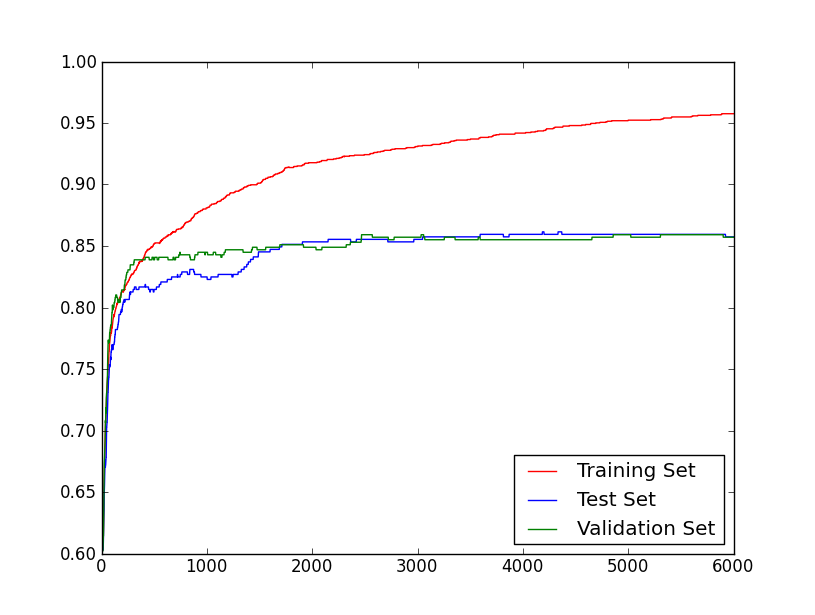
\includegraphics[width=.65\linewidth]{part4accuracy.png}
    \caption{The Accuracy Plot for Logistic Regression}
    \label{fig:logisticaccuracy}
\end{figure*}


\textbf{Regularization Parameters}\\
In this part, L2 regularization is used to prevent overfitting of the model. The reason behind choosing L2 regularization is because of the computational efficiency, as well as having a definite analytical solution.\\
In this problem, we have tuned the coefficient of the regularization, $\lamda$, using a linear search across a series of values and take coefficient with the highest accuracy for the validation set. We first searched across different magnitudes from $1^0$ to $1^{-4}$. Then after finding the optimal coefficient being 0.0001, we then did a grid search around 0.0001 and we found that a coefficient of 0.0005 produces the best result, with a validation set accuracy of $85.71\%$, a training accuracy of $95.75\%$ and a test accuracy of $85.74\%$.


\end{homeworkProblem}
\clearpage

%----------------------------------------------------------------------------------------
%	PROBLEM 5
%----------------------------------------------------------------------------------------

\begin{homeworkProblem}
\noindent \textit{Interpreting $\theta$ and I}\\

\begin{equation}
    \theta_0 + \theta_1I_1(x) + \theta_2I_2(x) + ... + \theta_nI_n(x) >thr   
\end{equation}
    



\textbf{Logistic Regression}\\
We can formulate logistic regression by the following: 
\begin{equation*}
    P(y^{(i)} = 1|x^{(i)},\theta) =  \frac{1}{1+e^{-\theta^Tx^{(i)}}}
\end{equation*}
\begin{equation*}
    P(y^{(i)} = 0|x^{(i)},\theta) =  \frac{e^{-\theta^Tx^{(i)}}}{1+e^{-\theta^Tx^{(i)}}}
\end{equation*}
which can be simpify to the following:
\begin{equation*}
    \frac{P(y^{(i)} = 1|x^{(i)},\theta)}{P(y^{(i)} = 0|x^{(i)},\theta)} = e^{\theta^Tx^{(i)}} > 1
\end{equation*}
 Then we can see that the decision boundary is characterized by the expression:
\begin{equation*}
    \theta^Tx^{(i)} = \theta_0 + \theta_1x_1 + \theta_2x_2 + ... + \theta_nx_n > 0
\end{equation*}

We know that in logistic regression, the $\theta$s represent the weights corresponding to each of the feature. The $x_i$ represents ith feature. In this case it will be the word and its presence in the headline. Note that every word is 1-hot encoding, with 1 representing presence of word and 0 representing absence of word, resulting in the threshold being 0.  As such, we can see that the $\theta$s in (5) correponds to $\theta^T$ in the decision boundary expression and that $I_n(x)$ is characterized by x_i.\\

\textbf{Naive Bayes}\\
We know that we can compute the log-odds of y = c using naive bayes. In our scenario, y will be whether a news headline is real or fake, with y = 1 being real and y = 0 being fake. From this fact, we can obtain the following expression:
\begin{equation*}
    \frac{P(y = c|x_1,...,x_p)}{P(y = c'|x_1,...,x_p)} > 1
\end{equation*}
Then, by computing the log probability, we have the following:
\begin{equation*}
    \begin{split}
        log\frac{P(y = c|x_1,...,x_p)}{P(y = c'|x_1,...,x_p)} &= log\frac{P(y = c)\Pi_{j}P(x_j|c)}{P(y = c')\Pi_{j}P(x_j|c')} > 0\\
                     &= log\frac{P(y = c)}{P(y = c')}+\sum_{j}log\frac{P(x_j|y = c)}{P(x_j|y = c')}\\
                     &= \beta_0 + \sum_j\beta_jx_j
    \end{split}
\end{equation*}
with
\begin{align*}
\beta_0 &= log\frac{P(y = c)}{P(y = c')}+\sum_{j}log\frac{P(x_j = 0|y = c)}{P(x_j = 0|y = c')}          &  \beta_j &= log\frac{P(x_j = 1|y = c)}{P(x_j = 1|y = c')}-log\frac{P(x_j = 0|y = c)}{P(x_j = 0|y = c')}  
\end{align*}
Similar to logistic regression, we can then say that the decision boundary of the naives bayes can be characterized by the following expression: 
\begin{equation*}
    \beta_0 + \sum_j\beta_jx_j > 0
\end{equation*}
We can then relate the $\beta_0 + \sum_j\beta_jx_j$ to (5). \\It is evident that $\beta$ corresponds to $\theta$ and $x_j$ corresponds to $I_j$.

\end{homeworkProblem}
\clearpage

%----------------------------------------------------------------------------------------
%	PROBLEM 6
%----------------------------------------------------------------------------------------

\begin{homeworkProblem}
\textbf{Part A)}\\
\noindent \textit{Displaying $\theta$ for Logistic Regression Model and their corresponding words with Stop Words}\\
%1. display a list of top 10 positive θs and negative θs
%2. How do these lists compare with those in part 3(a)? Do you notice any similarities or differences?
\textbf{10 words that Corresponds to Top 10 Positive $\theta$}\\


\begin{table}[!ht]
\begin{center}
 \begin{tabular}{||c c c||} 
 \hline
 Rank & Word & $\theta$  \\ [0.5ex] 
 \hline\hline
 1 & 2.831 & trumps  \\ 
 \hline
 2 & 1.680 & turnbull  \\
 \hline
 3 & 1.659 & says  \\
 \hline
 4 & 1.629 & us  \\
 \hline
 5 & 1.489 & korea \\ 
 \hline
 6 & 1.435 & north \\ 
 \hline 
 7 & 1.320 & australia\\
 \hline 
 8 & 1.275 & ban\\
 \hline
 9 & 1.266 & donald\\
 \hline 
 10 & 1.237 & debate\\ 
 \hline
\end{tabular}
\end{center}
\caption{Top 10 Positive $\theta$ and their Corresponding Words}
\label{table:stopwordspositive}
\end{table}


\textbf{10 words that Corresponds to Top 10 Negative $\theta$}\\

\begin{table}[!ht]
\begin{center}
 \begin{tabular}{||c c c||} 
 \hline
 Rank & Word & $\theta$  \\ [0.5ex] 
 \hline\hline
 1 & -2.148 & breaking  \\ 
 \hline
 2 & -2.073 & hillary  \\
 \hline
 3 & -1.914 & watch  \\
 \hline
 4 & -1.720 & just  \\
 \hline
 5 & -1.647 & black \\ 
 \hline
 6 & -1.587 & that \\ 
 \hline 
 7 & -1.417 & no\\
 \hline 
 8 & -1.368 & won\\
 \hline
 9 & -1.358 & victory\\
 \hline 
 10 & -1.337 & america\\ 
 \hline
\end{tabular}
\end{center}
\caption{Top 10 Negative $\theta$ and their Corresponding Words}
\label{table:stopwordsnegative}
\end{table}
\\
By comparing Table~\ref{table:stopwordspositive} \& Table~\ref{table:stopwordsnegative} to the list presented in 3(a), we can notice that the top 10 positive $\theta$ is similar to the list of words whose presence most strongly predicts that the news is real and that the top 10 negative $\theta$ is similar to the list of words whose presence most strongly predicts that the news is fake. In both cases, although the lists have overlaps with each other, there are still discrepancies in the entries, for example, words such as hillary is present in the logistic model but not the naives bayes model.


\newpage
\textbf{Part B)}\\
\noindent \textit{Displaying $\theta$ for Logistic Regression Model and their corresponding words with Stop Words}\\
\textbf{10 words that Corresponds to Top 10 Positive $\theta$}\\
\begin{table}[!ht]
\begin{center}
 \begin{tabular}{||c c c||} 
 \hline
 Rank & $\theta$ & Word  \\ [0.5ex] 
 \hline\hline
 1 & 2.831 & trumps  \\ 
 \hline
 2 & 1.680 & turnbull  \\
 \hline
 3 & 1.659 & says  \\
 \hline
 4 & 1.489 & korea  \\
 \hline
 5 & 1.435 & north \\ 
 \hline
 6 & 1.320 & australia \\ 
 \hline 
 7 & 1.2750 & ban\\
 \hline 
 8 & 1.266 & donald\\
 \hline
 9 & 1.237 & debate\\
 \hline 
 10 & 1.225 & tax\\ 
 \hline
\end{tabular}
\end{center}
\caption{Top 10 Positive $\theta$ and their Corresponding Words}
\label{table:nostopwordpositive}
\end{table}



\textbf{10 words that Corresponds to Top 10 Negative $\theta$}\\
\begin{table}[!ht]
\begin{center}
 \begin{tabular}{||c c c||} 
 \hline
 Rank & $\theta$ & Word  \\ [0.5ex] 
 \hline\hline
 1 & -2.148 & breaking  \\ 
 \hline
 2 & -2.073 & hillary  \\
 \hline
 3 & -1.914 & watch  \\
 \hline
 4 & -1.720 & just  \\
 \hline
 5 & -1.647 & black \\ 
 \hline
 6 & -1.368 & won \\ 
 \hline 
 7 & -1.358 & victory\\
 \hline 
 8 & -1.337  & america\\
 \hline
 9 & -1.300 & daily\\
 \hline 
 10 & -1.288 & new\\ 
 \hline
\end{tabular}
\caption{Top 10 Negative $\theta$ and their Corresponding Words}
\label{table:nostopwordsnegative}
\end{center}
\end{table}

By comparing Table~\ref{table:nostopwordpositive} \& Table~\ref{table:nostopwordsnegative} to the list presented in 3(b), we can notice that the top 10 positive $\theta$ is similar to the list of words whose presence most strongly predicts that the news is real and that the top 10 negative $\theta$ is similar to the list of words whose presence most strongly predicts that the news is fake. In both cases, although the lists have overlaps with each other, there are still discrepancies in the entries, for example, words such as hillary is present in the logistic model but not the naives bayes model.

\clearpage
\textbf{Part C)}\\
\noindent \textit{Magnitude of Logistic Regression Parameters}\\
Using the magnitude of logistic regression parameter to indicate the importance of a feature might not optimal in general because of the lack of normalization. If the features are not normalized, then there is a chance that features will be in different units and scales. As such, the largest weights may not due to the higest importance, but a result from different units. For example, a large weight may be correspond to a feature with smaller units relative to others, thus rendering the large weight misleading and vice versa. 
\\
However in this problem, it is reasonable to use the magnitude of logistic regression as a parameter to indicate the importance since all the words are normalized and that they are all measured in the same unit, with 1 being present in the headline and 0 being absent in the headline. 

\end{homeworkProblem}
\clearpage

%----------------------------------------------------------------------------------------
%	PROBLEM 7
%----------------------------------------------------------------------------------------

\begin{homeworkProblem}
\textbf{Part A)}\\
\noindent \textit{Train the decision tree classifier}\\

\begin{figure*}[!ht]
    \centering
    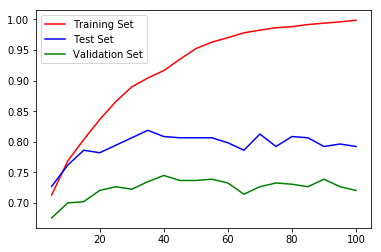
\includegraphics[width=.65\linewidth]{Part7Accuracy.png}
    \caption{The Accuracy Plot for Logistic Regression}
    \label{fig:Decisiontreeclassifier}
\end{figure*}

As shown from Fig~\ref{fig:Decisiontreeclassifier}, it can be seen that the overall accuracy for training set, test set and validation set are all increasing until the depth of the tree reached around 40. Afterwards, the accuracy of the training set continue to increase whereas the accuracy for the test and validation set fluctuated around 80\% and 70\% respectively. The best performance maximum depth of the decision tree is determined by selecting the highest accuracy on the validation set. As such, the optimal depth of the decision tree is said to be 40, as it produced a validation set with an accuracy of 74.49\%. Further, with this parameter, we have obtained a training accuracy of 91.64\% and a test accuracy of 80.85\%.\\
Aside from the depth, the criterion for this decision tree is set to be entropy, instead of the default gini. This is another way of splitting the information, and the purpose of using entropy is to maximize the mutual information at every split. This have increased the validation performance from $72.86\%$ to $73.27\%$.

\clearpage
\textbf{Part B)}\\
\noindent \textit{Extract and visualize the first two layers of the tree}\\
\begin{figure*}[!ht]
    \centering
    \includegraphics[width=.9\linewidth]{tree40.png}
    \caption{The Visualization of Decision Tree with a depth of 40}
    \label{fig:tree40}
\end{figure*}
*Note that after generating the 'dot.file' with the code, the dot file will have to be converted to png using the following command :
\begin{lstlisting}
from subprocess import check_call
check_call(['dot','-Tpng','InputFile.dot','-o','OutputFile.png'])
\end{lstlisting}
where 'InputFile.dot' should be the directory of which the dot file is created and the 'OutputFile.png' should be the directory and file name you wish to save the picture.

\clearpage
\begin{figure*}[!ht]
    \centering
    \includegraphics[width=.65\linewidth]{treetop2.png}
    \caption{The Visualization of the first 3 layers of the Decision Tree}
    \label{fig:treetop2}
\end{figure*}
\\

As seen in Fig~\ref{fig:treetop2}, the top features (words) determined by the Decision Tree is listed as the following: 

\begin{itemize}
\item the
\item donald
\item trumps
\item a
\item hillary
\item market
\end{itemize}
\\
\textbf{Decision Tree vs Naive Bayes}\\
When comparing the top words obtained from decision tree with the lists of words obtained from Naive Bayes classifier, we can see that all of the top words aside from 'market' is present in one of the lists. The word 'donald' and 'trumps' are present in the list of words whose absence most stronly predicts that the news is fake. The word 'the', 'a' and 'hillary' are present in the list of words whos absence most strongly predicts that the news is real. The overlapping of the words suggest that the top features obtained in the decision tree is mostly linked with the list of words whose absence strongly indicate the truth behind the headlines. 


\textbf{Decision Tree vs Logistic Regression}\\
When comparing the above list with Table~\ref{table:stopwordspositive}, we can see that the top words overlaps with the $\theta$. Specifically, the words donald and trumps are present in the top 10 positive $\theta$ and the word hillary is present in the top 10 negative $\theta$. Thus, there is still overlapping between decision tree and logistic regression to a certain degree. 


\clearpage
\textbf{Part C)}\\
\noindent \textit{Performance of your three classifiers on the training, validation, and test sets}\\
 \begin{table}[!ht]
\begin{center}
 \begin{tabular}{||c c c c||} 
 \hline
 Classifier & Training Accuracy & Validation Accuracy & Test Accuracy  \\ [0.5ex] 
 \hline\hline
 Logistic Regression & 92.39\% & 85.92\%  & 85.54\%\\ 
 \hline
 Naive Bayes & 96.89\% & 84.29\% & 86.15\%\\
 \hline
 Decision Tree & 91.64\% & 74.49\% & 80.85\%\\
 \hline
\end{tabular}
\end{center}
\caption{Performance of Each Classifier on Training, Validation and Test Set}
\label{table:classifierperformance}
\end{table}\\
*Note that the values obtained in Table ~\ref{table:classifierperformance} is found using the best performing parameters for each classifier, which is indicated by the highest accuracy in the validation set.\\
\\

It can be seen that the classifier that performed the best is Naive Bayes, as it has the highest test accuracy of $86.15\%$. The worst performing classifier is the Decision Tree, as it only has a test accuracy of $80.85\%$. It can also be noticed that decision tree overfits the training data the most, as it has a training accuracy of $91.64\%$ but only a validation accuracy of $74.49\%$, with an overall difference of $17.15\%$. This difference is the highest among the classifier, hence overfits the most because the model performs well on the training set but not so well on the validation and test set.  
\end{homeworkProblem}
\clearpage

%----------------------------------------------------------------------------------------
%	PROBLEM 8
%----------------------------------------------------------------------------------------

\begin{homeworkProblem}
\textbf{Part A)}\\
\noindent \textit{}\\
As we can observe in Figure~\ref{fig:treetop2}, the first split is the word 'the'.\\

\textbf{Method 1: Calculation by hand}\\
\textit{\underline{Step1: Compute Entropy H(Y)}}\\
We can obtain $P(T=real)$ & $P(T=fake)$ by counting:
\begin{equation*}
    P(T=real) = \frac{1377}{1377+908} = 0.602626\\
\end{equation*}
\begin{equation*}
    P(T=fake) = \frac{908}{1377+908} = 0.397374\\   
\end{equation*}

\begin{equation*}
    \begin{split}
        H(Y) &= -P(T=real) \times log_2{(P(T=real))} - P(T=real) \times log_2{(P(T=real))}\\
                                      &= - 0.602626*log_2{(0.602626)} - 0.397374*log_2{(0.397374)}\\
                                      &= 0.96939385
    \end{split}
\end{equation*}


\textit{\underline{Step2: Compute Conditional Entropy $H(Y|x_i)$}}\\
\begin{multline*}
    \begin{split}
        H(Y|x_i= the) = P(the= 1) &\times [-P(T=real|the=1) \times log_2{P(T=real|the=1)} - P(T=fake|the=1) \\&\times log_2{P(T=fake|the=1)}] +\\
        &P(the=0)\times[-P(T=real|the=0)\times log_2{P(T=real|the=0)} - P(T=fake|the=0) \\
        &\times log_2{P(T=fake|'the'=0)}]
    \end{split}
\end{multline*}
\begin{equation*}
    \begin{split}
    H(Y|x_i= the) &= 0.158424*[-0.290063*log_2{(0.290063)}-0.709937*log_2{(0.709937)}]\\
                  &+ 0.842576*[-0.661458*log_2{(0.661458)}-0.338542*log_2{(0.338542)}]\\
                  &= 0.915687902
    \end{split}
\end{equation*}


\textit{\underline{Step3: Compute Mutual Information $I(x_i;Y)$}}\\
\begin{equation*}
    \begin{split}
        I(x_i=the;Y) &= H(Y) - H(Y|x_i=the) \\
                      &= 0.96939385 - 0.915687902 \\
                      &= 0.053705948\\
    \end{split}
\end{equation*}

\textbf{Method 2: Calculation by Function}\\


\begin{lstlisting}
def H(realTrain,fakeTrain):
    '''
    This function computes the entropy of the label, that is H(T)
    '''
    Pr = len(realTrain)/(len(realTrain)+len(fakeTrain))
    Pf = 1.0 - Pr
    return - Pr*np.log2(Pr) - Pf*np.log2(Pf)

def condH(xi,realTrain,fakeTrain,Pr_xi1,Pf_xi1,Pr_xi0,Pf_xi0):
    '''
    Conditional Entropy H(T|xi)
    '''
    Pxi = 0
    for news in (realTrain+fakeTrain):
        if xi in news:
            Pxi += 1
    Pxi = Pxi/ (len(realTrain)+len(fakeTrain))
    result = Pxi*(- Pr_xi1*np.log2(Pr_xi1) - Pf_xi1*np.log2(Pf_xi1))
    print(Pr_xi0,Pf_xi0)
    result += (1.0-Pxi)*(- Pr_xi0*np.log2(Pr_xi0) - Pf_xi0*np.log2(Pf_xi0))
    return result
# get the first word from the decision tree
xi =allWords[clf.tree_.feature[0]]
# count the database
allWords, P_AllWordsReal, P_real, P_AllWordsFake, P_fake = NBCount(realTrain,fakeTrain,m,p)
Pr_xi1,Pf_xi1,Pr_xi0,Pf_xi0 = NBWord(xi,allWords,P_AllWordsReal,P_real, P_AllWordsFake,P_fake)
# compute mutual infotmaton
I = H(realTrain,fakeTrain) - condH(xi,realTrain,fakeTrain,Pr_xi1,Pf_xi1,Pr_xi0,Pf_xi0)
print xi,I
\end{lstlisting}\\
*Code used to generate the mutual information for the word 'the'.\\
\\
The mutual information of the word 'the': 0.0546294502518.\\
\\
Note: Compared with the value of 0.0546294502518, which is computed by the program, there is a slight difference of $2\%$ but this is reasonable since the truncation error of each step will accumulate. In this case, to guarantee the precision, we choose the result from function as our final value of mutual information, which is 0.0546294502518.\\





\clearpage
\textbf{Part B)}\\
\noindent \textit{}\\
\begin{table}[!ht]
\begin{center}
 \begin{tabular}{||c c||} 
 \hline
 Word (x_i) & I(x_i;Y) \\ [0.5ex] 
 \hline\hline
 donald & 0.04261  \\ 
 \hline
 trumps & 0.04616  \\
 \hline
 hillary & 0.03138  \\
 \hline
 us & 0.02017  \\
 \hline

 \hline
\end{tabular}
\end{center}
\caption{Computed $I(x_i;Y)$ for the successive words}
\label{table:wordvssplit}
\end{table}




\begin{lstlisting}
def H(realTrain,fakeTrain):
    '''
    This function computes the entropy of the label, that is H(T)
    '''
    Pr = len(realTrain)/(len(realTrain)+len(fakeTrain))
    Pf = 1.0 - Pr
    return - Pr*np.log2(Pr) - Pf*np.log2(Pf)
    

def condH(xi,realTrain,fakeTrain,Pr_xi1,Pf_xi1,Pr_xi0,Pf_xi0):
    '''
    H(T|xi)
    '''
    Pxi = 0
    for news in (realTrain+fakeTrain):
        if xi in news:
            Pxi += 1
    Pxi = Pxi/ (len(realTrain)+len(fakeTrain))
    result = Pxi*(- Pr_xi1*np.log2(Pr_xi1) - Pf_xi1*np.log2(Pf_xi1))
    print(Pr_xi0,Pf_xi0)
    result += (1.0-Pxi)*(- Pr_xi0*np.log2(Pr_xi0) - Pf_xi0*np.log2(Pf_xi0))
    return result
    
# get the next 4 words from the decision tree
for i in range(1,5):
    xi =allWords[clf.tree_.feature[i]]
    # count the database
    Pr_xi1,Pf_xi1,Pr_xi0,Pf_xi0 = NBWord(xi,allWords,P_AllWordsReal,P_real, P_AllWordsFake,P_fake)
    # compute mutual information
    I = H(realTrain,fakeTrain) - condH(xi,realTrain,fakeTrain,Pr_xi1,Pf_xi1,Pr_xi0,Pf_xi0)
    print i,xi,I 
\end{lstlisting}
\textit{*Code used to generate $I(x_i;Y)$ in Table~\ref{table:wordvssplit}}\\
    
As shown by Table~\ref{table:wordvssplit}, all of the successive variables (words) have a decrease of mutual information than the word 'the'. This is expected as decision tree prioritizes the words with the maximum mutual information. As a result, each split will provide the most information. 


\end{homeworkProblem}
\clearpage

%----------------------------------------------------------------------------------------



\end{document}